\documentclass[obeyspaces,aspectratio=43]{beamer}

\usetheme{bjeldbak}
\usepackage{ragged2e}
\usepackage{animate}
\newcommand{\columnsbegin}{\begin{columns}}
\newcommand{\columnsend}{\end{columns}}
\setbeamertemplate{caption}[numbered]
\setbeamertemplate{caption label separator}{:}
\setbeamercolor{caption name}{fg=normal text.fg}
\usepackage{amssymb,amsmath,fancyvrb}
\usepackage{ifxetex,ifluatex}
\usepackage{fixltx2e} % provides \textsubscript
\usepackage{lmodern}
\ifxetex
  \usepackage{fontspec,xltxtra,xunicode}
  \defaultfontfeatures{Mapping=tex-text,Scale=MatchLowercase}
  \newcommand{\euro}{€}
\else
  \ifluatex
    \usepackage{fontspec}
    \defaultfontfeatures{Mapping=tex-text,Scale=MatchLowercase}
    \newcommand{\euro}{€}
  \else
    \usepackage[T1]{fontenc}
    \usepackage[utf8]{inputenc}
      \fi
\fi
% use upquote if available, for straight quotes in verbatim environments
\IfFileExists{upquote.sty}{\usepackage{upquote}}{}
% use microtype if available
\IfFileExists{microtype.sty}{\usepackage{microtype}}{}
\usepackage{longtable,booktabs}
\usepackage{caption}
% These lines are needed to make table captions work with longtable:
\makeatletter
\def\fnum@table{\tablename~\thetable}
\makeatother

%\usepackage{hyperref}
\def\UrlBreaks{\do\/\do-}



\usepackage{bm}

% Comment these out if you don't want a slide with just the
% part/section/subsection/subsubsection title:
% \AtBeginPart{
%   \let\insertpartnumber\relax
%   \let\partname\relax
%   \frame{\partpage}
% }
% \AtBeginSection{
%   \let\insertsectionnumber\relax
%   \let\sectionname\relax
%   \frame{\sectionpage}
% }
% \AtBeginSubsection{
%   \let\insertsubsectionnumber\relax
%   \let\subsectionname\relax
%   \frame{\subsectionpage}
% }
\usepackage{tikz}
\usetikzlibrary{decorations.pathreplacing,calc}
\newcommand{\tikzmark}[1]{\tikz[overlay,remember picture] \node (#1) {};}

\setbeamersize{text margin left=2em,text margin right=2em}

% Make links footnotes instead of hotlinks:
\renewcommand{\href}[2]{#2\footnote{\url{#1}}}


\setlength{\parindent}{0pt}
\setlength{\parskip}{6pt plus 2pt minus 1pt}
\setlength{\emergencystretch}{3em}  % prevent overfull lines
\setcounter{secnumdepth}{0}
\providecommand{\tightlist}{%
  \setlength{\itemsep}{0pt}\setlength{\parskip}{0pt}}

\DeclareMathOperator*{\argmin}{arg\,min}

\newcommand{\twopartdef}[4]
{
  \left\{
    \begin{array}{ll}
      #1 & \mbox{if } #2 \\
      #3 & \mbox{if } #4
    \end{array}
  \right.
}

\newcommand{\twopartdefo}[3]
{
  \left\{
    \begin{array}{ll}
      #1 & \mbox{if } #2 \\
      #3 & \mbox{otherwise}
    \end{array}
  \right.
}

%gets rid of bottom navigation bars
\setbeamertemplate{footline}[frame number]{}

%gets rid of navigation symbols
\setbeamertemplate{navigation symbols}{}
\usebackgroundtemplate{
  \tikz[overlay,remember picture]
  \node[opacity=0.4, at=(current page.north east),anchor=north east] {
    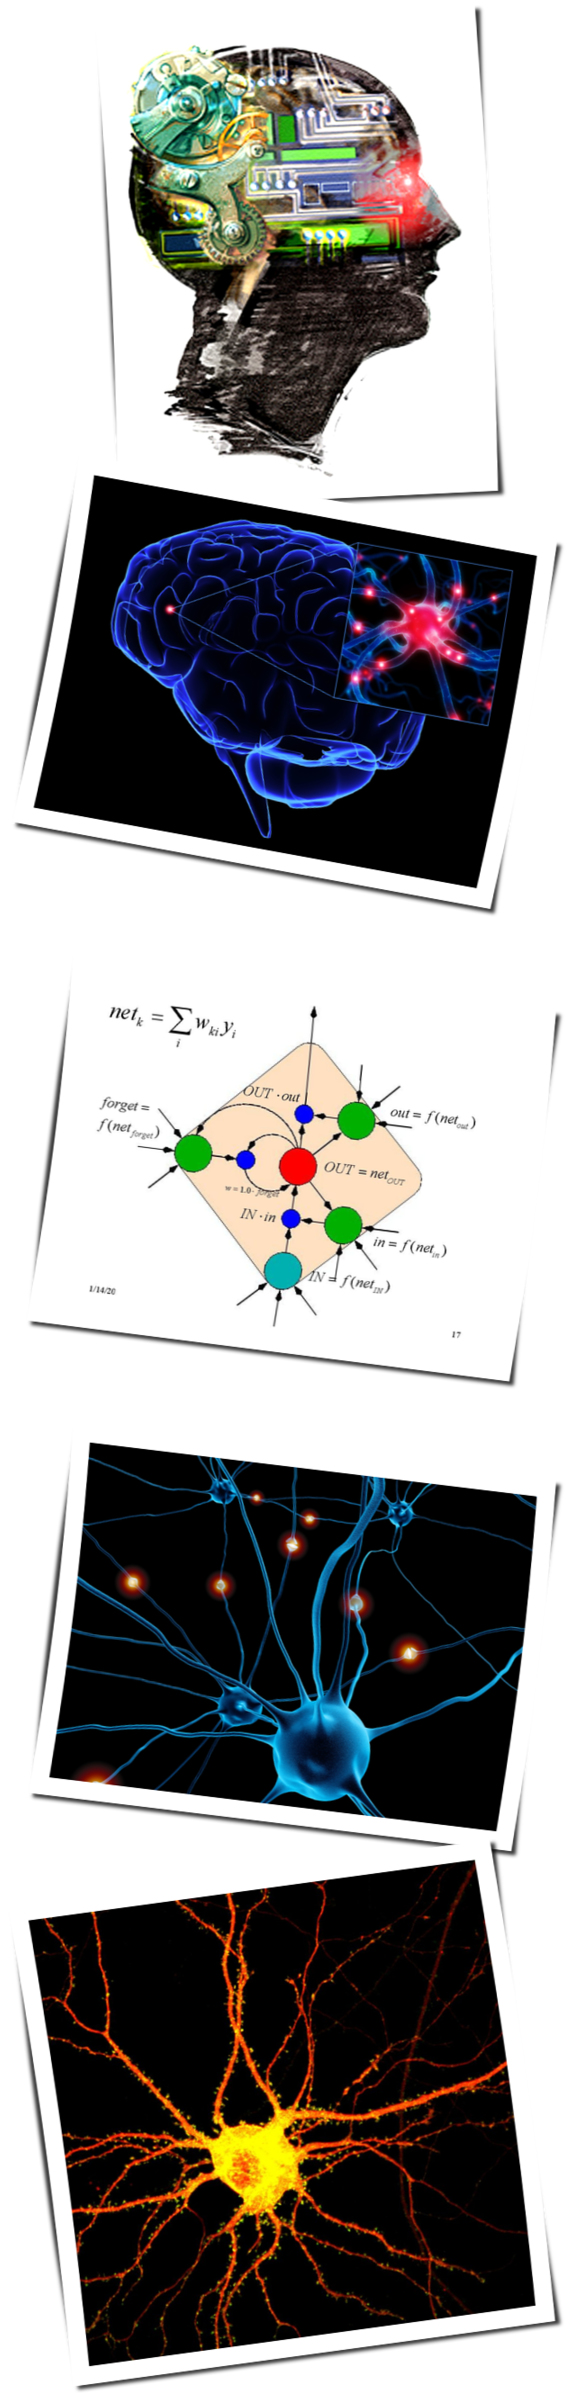
\includegraphics[width=0.17\paperwidth]{graphics/nn.jpg}};
}

\DeclareMathOperator*{\argmax}{arg\,max}


\newcommand{\vect}[1]{\boldsymbol{#1}} % Uncomment for BOLD vectors.

\title{A quick introduction to machine learning\\
Spyros Samothrakis\\
Senior Lecturer, IADS\\
University of Essex\\
MiSoC}
\author{June 22, 2022}
\date{}

\begin{document}
\frame{\titlepage}


\section{}\label{section}

\usebackgroundtemplate{

}

\section{Introduction}\label{introduction}

\begin{frame}{Welcome/course contents}

\begin{itemize}
\tightlist
\item
  What will this course cover?

  \begin{itemize}
  \tightlist
  \item
    Day 1: An intro to machine learning (ML)
  \item
    Day 1: ML labs
  \item
    Day 2: An intro to causal inference
  \item
    Day 2: ML and causal inference labs
  \end{itemize}
\item
  Textbooks?

  \begin{itemize}
  \item
    \href{http://www.cs.cmu.edu/~tom/mlbook.html}{Mitchell, T. M.
    (1997). Machine learning.}
  \item
    \href{https://www.microsoft.com/en-us/research/publication/pattern-recognition-machine-learning/}{Bishop,
    C. M. (2006). Pattern recognition and machine learning. springer.}
  \item
    \href{http://www.stat.cmu.edu/~larry/all-of-statistics/index.html}{Wasserman,
    L. (2013). All of statistics: a concise course in statistical
    inference. Springer Science \& Business Media.}
  \end{itemize}
\end{itemize}

\end{frame}

\begin{frame}{Better science through data}

\href{http://languagelog.ldc.upenn.edu/myl/JimGrayOnE-Science.pdf}{Hey,
Tony, Stewart Tansley, and Kristin M. Tolle. ``Jim Gray on eScience: a
transformed scientific method.'' (2009).}

\begin{itemize}
\tightlist
\item
  Thousand years ago: empirical branch

  \begin{itemize}
  \tightlist
  \item
    You observed stuff and you wrote down about it
  \end{itemize}
\item
  Last few hundred years: theoretical branch

  \begin{itemize}
  \tightlist
  \item
    Equations of gravity, equations of electromagnetism
  \end{itemize}
\item
  Last few decades: computational branch

  \begin{itemize}
  \tightlist
  \item
    Modelling at the micro level, observing at the macro level
  \end{itemize}
\item
  Today: data exploration

  \begin{itemize}
  \tightlist
  \item
    Let machines create models using vast amounts of data
  \end{itemize}
\end{itemize}

\end{frame}

\begin{frame}{Better business through data}

\begin{itemize}
\tightlist
\item
  There was a report by Mckinsey
\end{itemize}

\href{http://www.mckinsey.com/business-functions/digital-mckinsey/our-insights/big-data-the-next-frontier-for-innovation}{Manyika,
J., Chui, M., Brown, B., Bughin, J., Dobbs, R., Roxburgh, C., \& Hung
Byers, A. (2011). Big data: The next frontier for innovation,
competition, and productivity. McKinsey Global Institute.}

\begin{itemize}
\tightlist
\item
  Urges everyone to monetise ``Big Data''
\item
  Use the data provided within your organisation to gain insights
\item
  Has some numbers as to how much this is worth
\item
  Proposes a number of methods, most of them associated with machine
  learning and databases
\end{itemize}

\end{frame}

\begin{frame}{Why is it popular now?}

\begin{itemize}
\item
  \textbf{Algorithms + data + tools}
\item
  \href{http://projecteuclid.org/download/pdf_1/euclid.ss/1009213726\%20}{Breiman,
  L. (2001). Statistical modeling: The two cultures (with comments and a
  rejoinder by the author). Statistical science, 16(3), 199-231.}
\item
  \href{https://www.tkm.kit.edu/downloads/TKM1_2011_more_is_different_PWA.pdf}{Anderson,
  P. W. (1972). More is different. Science, 177(4047), 393-396.}
\item
  \href{https://www.jmlr.org/papers/volume12/pedregosa11a/pedregosa11a.pdf}{Pedregosa,
  et.al. (2011). Scikit-learn: Machine learning in Python. the Journal
  of machine Learning research, 12, 2825-2830.}
\end{itemize}

\end{frame}

\begin{frame}{What will we cover?}

\begin{itemize}
\tightlist
\item
  ML background

  \begin{itemize}
  \tightlist
  \item
    \emph{Supervised learning}

    \begin{itemize}
    \tightlist
    \item
      \emph{Regression}
    \item
      \emph{Classification}
    \end{itemize}
  \item
    Understanding basic modelling
  \item
    Confirming your model is sane
  \item
    Tuning your model
  \item
    \textbf{All within a very applied setting}
  \end{itemize}
\item
  Tools

  \begin{itemize}
  \tightlist
  \item
    Numpy
  \item
    Scikit-learn
  \end{itemize}
\end{itemize}

\end{frame}

\begin{frame}{What is supervised learning?}

\begin{itemize}
\tightlist
\item
  Imagine someone gives you data from a group of smokers

  \begin{itemize}
  \tightlist
  \item
    What is their life expectancy?
  \end{itemize}
\item
  We are given inputs \(x_0, x_1...x_n\) and we are looking to predict
  \(y\)
\item
  The problem alludes to certain statistical concepts
\item
  Let's plot some imaginary data
\end{itemize}

\end{frame}

\begin{frame}{Regression - link the dots (1)}

\includegraphics[trim={0 0 0 0},clip,width = 0.9\textwidth]{./code/cropped/{intra_spiral_50-crop}.jpg}

\end{frame}

\begin{frame}{Regression - link the dots (2)}

\includegraphics[trim={0 0 0 0},clip,width = 0.9\textwidth]{./code/cropped/{intra_spiral_100-crop}.jpg}

\end{frame}

\begin{frame}{Regression - link the dots (3)}

\includegraphics[trim={0 0 0 0},clip,width = 0.9\textwidth]{./code/cropped/{intra_spiral_200-crop}.jpg}

\end{frame}

\begin{frame}{Regression - link the dots (4)}

\includegraphics[trim={0 0 0 0},clip,width = 0.9\textwidth]{./code/cropped/{intra_spiral_500-crop}.jpg}

\end{frame}

\begin{frame}{Regression - link the dots (5)}

\includegraphics[trim={0 0 0 0},clip,width = 0.9\textwidth]{./code/cropped/{intra_spiral_1000-crop}.jpg}

\end{frame}

\begin{frame}{Regression - link the dots (6)}

\includegraphics[trim={0 0 0 0},clip,width = 0.9\textwidth]{./code/cropped/{intra_spiral_10000-crop}.jpg}

\end{frame}

\begin{frame}{Classification - draw a boundary (1)}

\includegraphics[trim={0 0 0 0},clip,width = 0.9\textwidth]{./code/cropped/{intra_spiral_50_class-crop}.jpg}

\end{frame}

\begin{frame}{Classification - draw a boundary (2)}

\includegraphics[trim={0 0 0 0},clip,width = 0.9\textwidth]{./code/cropped/{intra_spiral_100_class-crop}.jpg}

\end{frame}

\begin{frame}{Classification - draw a boundary (3)}

\includegraphics[trim={0 0 0 0},clip,width = 0.9\textwidth]{./code/cropped/{intra_spiral_200_class-crop}.jpg}

\end{frame}

\begin{frame}{Classification - draw a boundary (4)}

\includegraphics[trim={0 0 0 0},clip,width = 0.9\textwidth]{./code/cropped/{intra_spiral_500_class-crop}.jpg}

\end{frame}

\begin{frame}{Classification - draw a boundary (5)}

\includegraphics[trim={0 0 0 0},clip,width = 0.9\textwidth]{./code/cropped/{intra_spiral_1000_class-crop}.jpg}

\end{frame}

\begin{frame}{Classification - draw a boundary (6)}

\includegraphics[trim={0 0 0 0},clip,width = 0.9\textwidth]{./code/cropped/{intra_spiral_10000_class-crop}.jpg}

\end{frame}

\begin{frame}{Full data}

\includegraphics[trim={0 0 0 0},clip,width = 0.9\textwidth]{./code/cropped/{extra_spiral-crop}.jpg}

\end{frame}

\begin{frame}{Intuition (1)}

\href{https://www.manning.com/books/deep-learning-with-python}{Chollet,
F. (2018). Deep learning with Python (Vol. 361). New York: Manning.}

\includegraphics[trim={0 0 0 0},clip,width = 0.9\textwidth]{./graphics/{programming}.jpeg}

\end{frame}

\begin{frame}{Intuition (2)}

\begin{itemize}
\tightlist
\item
  That's it - we are given data, and we need to come up with an
  algorithm to join it up -- but in high dimensions

  \begin{itemize}
  \tightlist
  \item
    Can can be binary, categorical, real-valued - more on this later
  \end{itemize}
\item
  How well well a function joins the data is called the ``loss''
\item
  Multiple solutions exist, so a loss function must take into account
  concepts other than pure fit
\end{itemize}

\end{frame}

\begin{frame}{Vs Causality}

\begin{itemize}
\tightlist
\item
  Imagine someone gives you data from a group of smokers

  \begin{itemize}
  \tightlist
  \item
    What is their life expectancy?
  \item
    \textbf{Is smoking bad for you?}
  \end{itemize}
\item
  You could potentially just do predictions using correlations

  \begin{itemize}
  \tightlist
  \item
    What if there was a gene that caused early death and also made you
    like smoking?
  \item
    More on this tomorrow
  \end{itemize}
\end{itemize}

\end{frame}

\section{Some algorithms}\label{some-algorithms}

\begin{frame}{Linear regression}

\begin{itemize}
\tightlist
\item
  Linear and logistic regression

  \begin{itemize}
  \tightlist
  \item
    Logistic regression does classification
  \end{itemize}
\item
  You just assume everything is a line
\item
  \(f(x) = wx + b\)
\end{itemize}

\end{frame}

\begin{frame}{Example (Linear regression)}

\includegraphics[trim={0 0 0 0},clip,width = 0.9\textwidth]{./code/cropped/{reg_intra_spiral_200_LinearRegression-crop}.jpg}

\end{frame}

\begin{frame}{Example (Linear regression)}

\includegraphics[trim={0 0 0 0},clip,width = 0.7\textwidth]{./code/cropped/{reg_intra_spiral_2000_LinearRegression-crop}.jpg}

\(f(x) = 0.9x + 9.1\)

\end{frame}

\begin{frame}{Example (Decision tree)}

\includegraphics[trim={0 0 0 0},clip,width = 0.9\textwidth]{./code/cropped/{reg_intra_spiral_200_DecisionTreeRegressor-crop}.jpg}

\end{frame}

\begin{frame}{Example (Decision tree)}

\includegraphics[trim={0 0 0 0},clip,width = 0.9\textwidth]{./code/cropped/{reg_intra_spiral_2000_DecisionTreeRegressor-crop}.jpg}

\end{frame}

\begin{frame}{Example (Decision tree --- internal)}

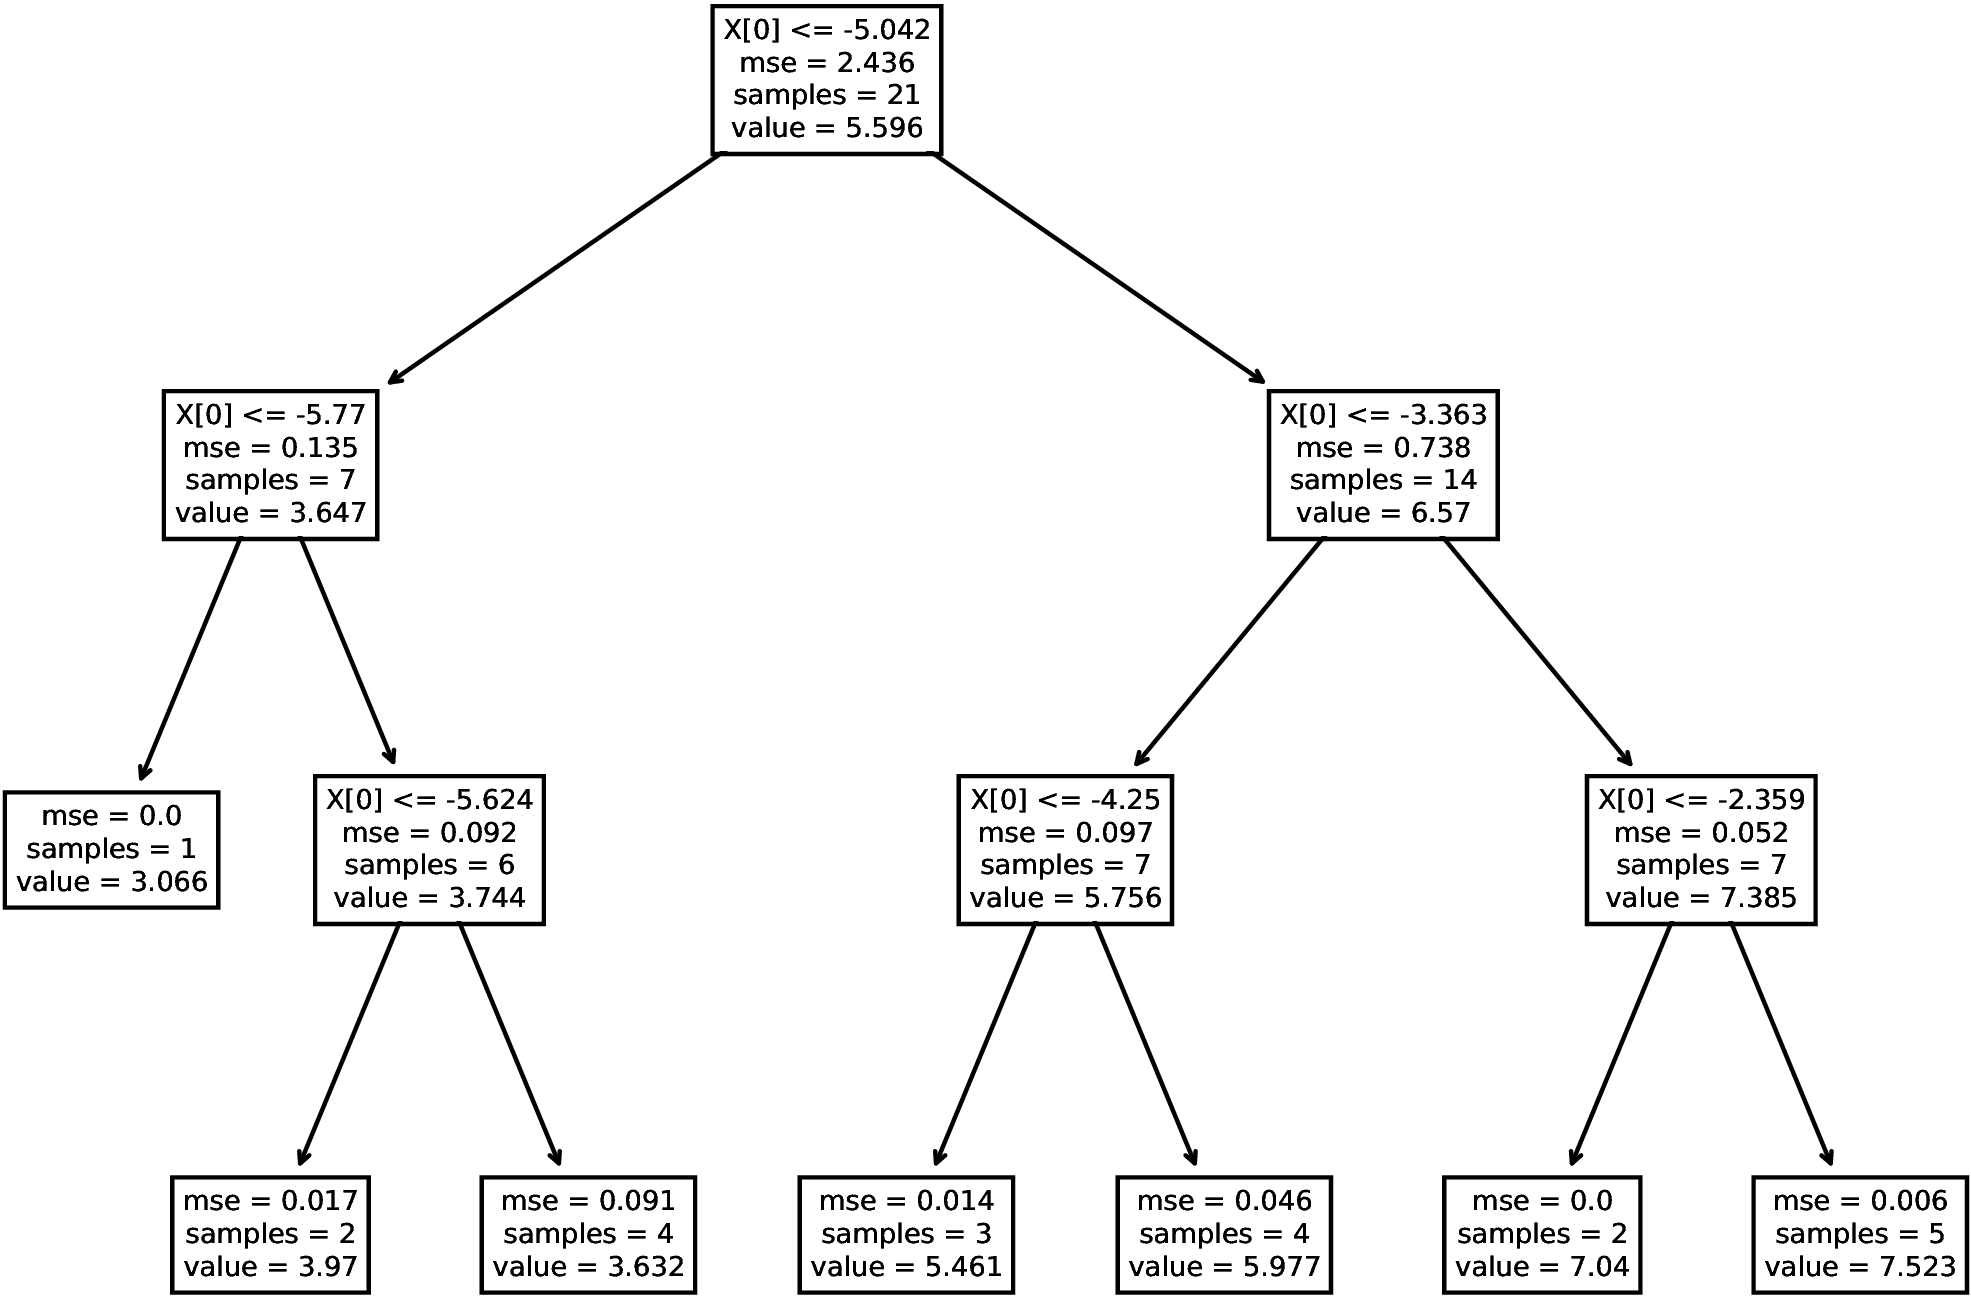
\includegraphics[trim={0 0 0 0},clip,width = 0.9\textwidth]{./graphics/tree_onedim.png}

\end{frame}

\begin{frame}{Example (Random forest)}

\includegraphics[trim={0 0 0 0},clip,width = 0.9\textwidth]{./code/cropped/{reg_intra_spiral_2000_RandomForestRegressor-crop}.jpg}

\end{frame}

\begin{frame}{Example (Random forest)}

\includegraphics[trim={0 0 0 0},clip,width = 0.9\textwidth]{./code/cropped/{reg_intra_spiral_2000_RandomForestRegressor-crop}.jpg}

\end{frame}

\begin{frame}{Example (Random forest)}

\includegraphics[trim={0 0 0 0},clip,width = 0.9\textwidth]{./code/cropped/{reg_intra_spiral_2000_CatBoostRegressor-crop}.jpg}

\end{frame}

\begin{frame}{Example (Gradient boosting)}

\includegraphics[trim={0 0 0 0},clip,width = 0.9\textwidth]{./code/cropped/{reg_intra_spiral_2000_CatBoostRegressor-crop}.jpg}

\end{frame}

\begin{frame}{Classification (Logistic regression)}

\includegraphics[trim={0 0 0 0},clip,width = 0.9\textwidth]{./code/cropped/{class_spiral_LogisticRegression}.png}

\end{frame}

\begin{frame}{Classification (Decision trees)}

\includegraphics[trim={0 0 0 0},clip,width = 0.9\textwidth]{./code/cropped/{class_spiral_DecisionTreeClassifier}.png}

\end{frame}

\begin{frame}{Classification (Random forests)}

\includegraphics[trim={0 0 0 0},clip,width = 0.9\textwidth]{./code/cropped/{class_spiral_RandomForestClassifier}.png}

\end{frame}

\section{Higher dimensions}\label{higher-dimensions}

\begin{frame}{Data dimensionality}

\begin{itemize}
\tightlist
\item
  Until now we have seen input data of 1 (for regression) or two (for
  classification) dimensions
\item
  How about higher dimensional data?

  \begin{itemize}
  \tightlist
  \item
    Some times data can have millions of features
  \end{itemize}
\item
  Let's examine more high dimensional dataset
\item
  Visualisation becomes harder
\end{itemize}

\end{frame}

\begin{frame}{Diabetes Classification}

\tiny

\begin{longtable}[c]{@{}ll@{}}
\toprule
Feature & Description\tabularnewline
\midrule
\endhead
\(X_0\) & Pregnancies: Number of times pregnant\tabularnewline
\(X_1\) & Glucose: Plasma glucose concentration\tabularnewline
\(X_2\) & BloodPressure: Diastolic blood pressure (mm Hg)\tabularnewline
\(X_3\) & SkinThickness: Triceps skin fold thickness (mm)\tabularnewline
\(X_4\) & Insulin: 2-Hour serum insulin (mu U/ml)\tabularnewline
\(X_5\) & BMI: Body mass index (weight in kg/(height in
m)\^{}2)\tabularnewline
\(X_6\) & DiabetesPedigreeFunction: Diabetes pedigree
function\tabularnewline
\(X_7\) & Age: Age (years)\tabularnewline
\(y\) & Outcome: Has diabetes (0 or 1)\tabularnewline
\bottomrule
\end{longtable}

\url{https://www.kaggle.com/mathchi/diabetes-data-set}

\end{frame}

\begin{frame}{How does the data look like?}

\center
\tiny

\begin{tabular}{lrrrrrrrr}
\toprule
{} &  Pregnancies &  Glucose &  BloodPressure &  SkinThickness &  Insulin &   BMI &  DPF &  Age \\
\midrule
0 &            6 &      148 &             72 &             35 &        0 & 33.60 &                      0.63 &   50 \\
1 &            1 &       85 &             66 &             29 &        0 & 26.60 &                      0.35 &   31 \\
2 &            8 &      183 &             64 &              0 &        0 & 23.30 &                      0.67 &   32 \\
3 &            1 &       89 &             66 &             23 &       94 & 28.10 &                      0.17 &   21 \\
4 &            0 &      137 &             40 &             35 &      168 & 43.10 &                      2.29 &   33 \\
\bottomrule
\end{tabular}

\begin{tabular}{lr}
\toprule
{} &  y \\
\midrule
0 &        1 \\
1 &        0 \\
2 &        1 \\
3 &        0 \\
4 &        1 \\
\bottomrule
\end{tabular}

\end{frame}

\begin{frame}{Decision Tree}

\includegraphics[trim={0 0 0 0},clip,width = 0.9\textwidth]{./graphics/{tree_class_diab}.png}

\end{frame}

\begin{frame}{Diabetes regression}

\href{https://scikit-learn.org/stable/datasets/toy_dataset.html\#diabetes-dataset}{Efron,
B., Hastie, T., Johnstone, I., \& Tibshirani, R. (2004). Least angle
regression. Annals of statistics, 32(2), 407-499.}

\tiny

\begin{longtable}[c]{@{}ll@{}}
\toprule
Feature & Description\tabularnewline
\midrule
\endhead
\(X_0\) & age in years\tabularnewline
\(X_1\) & sex\tabularnewline
\(X_2\) & bmi body mass index\tabularnewline
\(X_3\) & bp average blood pressure\tabularnewline
\(X_4\) & s1 tc, total serum cholesterol\tabularnewline
\(X_5\) & s2 ldl, low-density lipoproteins\tabularnewline
\(X_6\) & s3 hdl, high-density lipoproteins\tabularnewline
\(X_7\) & s4 tch, total cholesterol / HDL\tabularnewline
\(X_8\) & s5 ltg, possibly log of serum triglycerides
level\tabularnewline
\(X_9\) & s6 glu, blood sugar level\tabularnewline
\(y\) & disease progression one year after baseline\tabularnewline
\bottomrule
\end{longtable}

\end{frame}

\begin{frame}{Let's see the real data values}

\tiny
\center

\begin{tabular}{lrrrrrrrrrr}
\toprule                                                                                                                                                                      
{} &   age &   sex &   bmi &    bp &    s1 &    s2 &    s3 &    s4 &    s5 &    s6 \\                                                                                         
\midrule                                                                                                                                                                      
0 &  0.04 &  0.05 &  0.06 &  0.02 & -0.04 & -0.03 & -0.04 & -0.00 &  0.02 & -0.02 \\                                                                                          
1 & -0.00 & -0.04 & -0.05 & -0.03 & -0.01 & -0.02 &  0.07 & -0.04 & -0.07 & -0.09 \\                                                                                          
2 &  0.09 &  0.05 &  0.04 & -0.01 & -0.05 & -0.03 & -0.03 & -0.00 &  0.00 & -0.03 \\                                                                                          
3 & -0.09 & -0.04 & -0.01 & -0.04 &  0.01 &  0.02 & -0.04 &  0.03 &  0.02 & -0.01 \\                                                                                          
4 &  0.01 & -0.04 & -0.04 &  0.02 &  0.00 &  0.02 &  0.01 & -0.00 & -0.03 & -0.05 \\                                                                                          
\bottomrule                                                                                                                                                                   
\end{tabular}

``Note: Each of these 10 feature variables have been mean centered and
scaled by the standard deviation times n\_samples (i.e.~the sum of
squares of each column totals 1).''

\begin{tabular}{lr}
\toprule                                                                                                                                                                      
{} &  y \\                                                                                                                                                               
\midrule                                                                                                                                                                      
0 &  151.00 \\                                                                                                                                                                
1 &   75.00 \\                                                                                                                                                                
2 &  141.00 \\                                                                                                                                                                
3 &  206.00 \\                                                                                                                                                                
4 &  135.00 \\                                                                                                                                                                
\bottomrule                                                                                                                                                                   
\end{tabular}

\end{frame}

\begin{frame}{Linear regression}

\(y = -210x_0 -5036x_1 + 10916x_2 + 6812x_3  -16635x_4 10011x_5 + 2121x_6 + 3718x_7 +  15776x8 + 1420x_{9} + 152\)

\end{frame}

\section{Testing}\label{testing}

\begin{frame}{Quality assessment}

\begin{itemize}
\tightlist
\item
  In lower dimensions, the visualisations we did provided some insights
  to the quality of our methods

  \begin{itemize}
  \tightlist
  \item
    This is impossible in higher dimensions
  \end{itemize}
\item
  We need to measure some kind of metric that denotes quality of fit
\end{itemize}

\end{frame}

\begin{frame}{Metrics}

\begin{itemize}
\tightlist
\item
  For regression,

  \begin{itemize}
  \tightlist
  \item
    Mean Squared Error
  \item
    Mean Absolute Error
  \end{itemize}
\item
  For classification

  \begin{itemize}
  \tightlist
  \item
    Accuracy
  \item
    Mean Squared Error
  \item
    Cross-entropy loss
  \item
    AUC
  \end{itemize}
\item
  Each one has different benefits, e.g.~absolute errors tend to be more
  robust to outliers
\end{itemize}

\end{frame}

\begin{frame}{Accuracy}

\begin{itemize}
\tightlist
\item
  Our model is \(\hat{f}(x)\), \(x\) are examples, \(y\) is outcome
\item
  Accuracy is the obvious one

  \begin{itemize}
  \tightlist
  \item
    \(\mathit{accuracy} = \frac{1} {N} \sum\limits_{i=0}^{N-1}(y_i = \hat{f}(x) )\)
  \item
    The higher the accuracy the better
  \end{itemize}
\item
  What if the dataset is unbalanced - how informative is accuracy then?
\item
  There are multiple score functions

  \begin{itemize}
  \tightlist
  \item
    Use the one appropriate for your problem
  \end{itemize}
\end{itemize}

\end{frame}

\begin{frame}{Mean Squared Error (MSE)}

\begin{itemize}
\tightlist
\item
  Our model is \(\hat{f}(x)\), \(x\) are examples, \(y\) is outcome

  \begin{itemize}
  \tightlist
  \item
    \(MSE = \frac{1} {N} \sum\limits_{i = 1}^N \left( y_{i} - \hat{f}(x_{i}) \right)^2\)
  \end{itemize}
\end{itemize}

\end{frame}

\begin{frame}{Train/validation/test split}

\begin{itemize}
\item
  Basic idea: split your data into three portions
\item
  \begin{enumerate}
  \def\labelenumi{(\alph{enumi})}
  \tightlist
  \item
    train, you used that to train your classifier/regressor
  \end{enumerate}
\item
  \begin{enumerate}
  \def\labelenumi{(\alph{enumi})}
  \setcounter{enumi}{1}
  \tightlist
  \item
    validation, you use that to assess the quality of your method,
    retraining as you see fit
  \end{enumerate}
\item
  \begin{enumerate}
  \def\labelenumi{(\alph{enumi})}
  \setcounter{enumi}{2}
  \tightlist
  \item
    test, you report results on this
  \end{enumerate}
\item
  Common split is 60\%/20\%/20\%
\end{itemize}

\end{frame}

\begin{frame}{Cross validation}

\begin{itemize}
\tightlist
\item
  How about we split our data into multiple validation sets and find the
  mean?

  \begin{itemize}
  \tightlist
  \item
    Instead of having just one split train/test split, we can have
    multiple
  \end{itemize}
\item
  Colloquially goes by names like 5-fold CV, 10-fold CV
\item
  There are multiple ways of doing the sampling to create
  training/validation sets, we will focus on only one
\end{itemize}

\end{frame}

\begin{frame}{Pictorial depiction of 5-fold CV}

\href{https://scikit-learn.org/stable/_images/grid_search_cross_validation.png}{Copied
from SKlearns website}

\includegraphics[trim={0 0 0 0},clip,width = 0.8\textwidth]{./graphics/{grid_search_cross_validation}.png}

\end{frame}

\section{Tuning}\label{tuning}

\begin{frame}{Why tune?}

\begin{itemize}
\tightlist
\item
  Your data has peculiarities
\item
  You need to ``calibrate'' your algorithm with these peculiarities
\item
  Tuning properly will have a significant effect on cross-validation
  scores

  \begin{itemize}
  \tightlist
  \item
    \ldots{} and hence the quality of learning
  \end{itemize}
\end{itemize}

\end{frame}

\begin{frame}{Hyperparameters}

\begin{itemize}
\tightlist
\item
  Called hyperparameters (vs parameters) as they influence how the
  modelling is done (vs the direct modeling)

  \begin{itemize}
  \tightlist
  \item
    How many trees?
  \item
    Tree depth?
  \item
    Maximum tree size
  \item
    l2 regularisation?
  \end{itemize}
\item
  vs parameters (e.g.~weights in linear regression)
\end{itemize}

\end{frame}

\begin{frame}{We need to look for optimal parameters}

\begin{itemize}
\tightlist
\item
  Computationally expensive
\item
  We can do this either by searching both the classifier/regressor space
  and their parameters
\item
  Grid search

  \begin{itemize}
  \tightlist
  \item
    More than one parameter, we exhaustively search
  \end{itemize}
\end{itemize}

\end{frame}

\begin{frame}{Example using linear regression}

\tiny

\begin{longtable}[c]{@{}llll@{}}
\toprule
alpha & scores & mean & std\tabularnewline
\midrule
\endhead
0.0001 & {[}2782, 3032, 3226, 3003, 2917{]} & 2992.1772 &
145.5645\tabularnewline
0.0001 & {[}2783, 3032, 3223, 3002, 2920{]} & 2992.0154 &
143.9139\tabularnewline
0.0002 & {[}2785, 3032, 3218, 3001, 2923{]} & 2991.8400 &
141.7267\tabularnewline
0.0007 & {[}2812, 3042, 3186, 3002, 2945{]} & 2997.5634 &
122.1458\tabularnewline
0.0009 & {[}2818, 3042, 3179, 2992, 2946{]} & 2995.3784 &
117.9862\tabularnewline
0.0012 & {[}2827, 3043, 3178, 2978, 2947{]} & 2994.6426 &
115.5067\tabularnewline
0.0037 & {[}2884, 3060, 3190, 2895, 2968{]} & 2999.3816 &
114.1540\tabularnewline
0.0049 & {[}2918, 3079, 3201, 2869, 2985{]} & 3010.3321 &
118.4097\tabularnewline
0.0065 & {[}2938, 3111, 3215, 2856, 3017{]} & 3027.3294 &
126.2295\tabularnewline
0.0085 & {[}2966, 3152, 3219, 2859, 3057{]} & 3050.5713 &
128.2733\tabularnewline
0.0113 & {[}3014, 3212, 3236, 2872, 3113{]} & 3089.2555 &
134.1712\tabularnewline
0.0149 & {[}3028, 3292, 3279, 2918, 3201{]} & 3143.7112 &
146.9126\tabularnewline
0.0196 & {[}3040, 3366, 3358, 2970, 3289{]} & 3204.6848 &
166.7447\tabularnewline
0.0259 & {[}3082, 3493, 3484, 3074, 3435{]} & 3313.4750 &
193.2530\tabularnewline
0.0342 & {[}3206, 3706, 3681, 3237, 3678{]} & 3501.7398 &
229.0676\tabularnewline
0.0452 & {[}3434, 4030, 3972, 3448, 4037{]} & 3784.1217 &
281.4318\tabularnewline
0.0597 & {[}3801, 4573, 4447, 3745, 4545{]} & 4222.0278 &
369.6680\tabularnewline
0.0788 & {[}4401, 5460, 5212, 4299, 5425{]} & 4959.4742 &
505.7819\tabularnewline
0.1040 & {[}5211, 6521, 6262, 5200, 6486{]} & 5935.8770 &
603.2078\tabularnewline
0.1374 & {[}5353, 6521, 6262, 5290, 6486{]} & 5982.4134 &
547.2524\tabularnewline
\bottomrule
\end{longtable}

\end{frame}

\begin{frame}{What do you observer?}

\begin{itemize}
\tightlist
\item
  Properly tuning your model can have a huge impact!
\end{itemize}

\end{frame}

\section{Wrapping up}\label{wrapping-up}

\begin{frame}{Wrapping up}

\begin{itemize}
\tightlist
\item
  You get data from somewhere
\item
  ML will help you predict certain targets
\item
  Data can be noisy
\item
  You might need to pre-process it
\item
  The more data the better
\item
  Choosing the right classifier/regressor is important

  \begin{itemize}
  \tightlist
  \item
    Cross-validate and test
  \end{itemize}
\end{itemize}

\end{frame}

\end{document}
